\documentclass[aspectratio=169, table]{beamer}

\usepackage{array}
\usepackage{colortbl}
\usepackage{tabularx}
\usepackage{xcolor}
\usepackage{tikz}
\usetikzlibrary{arrows.meta, positioning, calc, fit}

\makeatletter
\def\input@path{{../theme/}}
\makeatother
\graphicspath{{../theme/}{../../figures/}}
\usetheme{Pradita}

\newcommand{\sectionframe}[1]{%
  \begin{frame}{\hfill}
    \centering
    \Huge{\textbf{#1}}
  \end{frame}
}

\newcommand{\takeaway}[1]{%
  \vspace{4pt}
  {\footnotesize #1}
}

\title{\huge Lapisan Strategi\\
  \vspace{8pt}
  pada ArchiMate}
\subtitle{IT30713 - Enterprise \& Platform Architecture}
\author{\textbf{Alfa Yohannis}}
\date{13 Juni 2026}

\begin{document}

\frame{\titlepage}

\begin{frame}[fragile]
  \frametitle{Contents}
  \vspace{20pt}
  \begin{columns}[t]
    \column{0.5\textwidth}
    \tableofcontents[sections={1-4}]

    \column{0.5\textwidth}
    \tableofcontents[sections={5-8}]
  \end{columns}
\end{frame}

\begin{frame}{\hfill}
  \centering
  \Huge{\textbf{Sasaran sudah jelas---lalu strategi apa yang dipilih?}}
\end{frame}

% ============================================================
\section{Orientasi Bab}
\sectionframe{Orientasi Bab}

\begin{frame}{Tujuan Pembelajaran}
  \vspace{8pt}
  \begin{itemize}
    \item Menjelaskan elemen \textbf{lapisan strategi} ArchiMate: sumber daya
          (\emph{resource}), kapabilitas (\emph{capability}), arah tindakan
          (\emph{course of action}), dan \emph{value stream}.
    \item Membaca \textbf{model bisnis} dan \emph{operating model} untuk memilih
          arah tindakan strategis organisasi studi kasus.
    \item Menyusun \textbf{visi arsitektur} dan \emph{roadmap} dengan
          \textbf{TOGAF-lite} dan ADM (\emph{Architecture Development Method}).
    \item Merancang \textbf{strategi pencarian pustaka} dan bibliografi awal
          yang mendukung argumen strategis makalah.
  \end{itemize}
  \takeaway{Arah sesi: dari ``mengapa'' (motivasi) menuju ``strategi apa''
  yang dipilih dan mengapa.}
\end{frame}

\begin{frame}{Ringkasan Awal Bab}
  \vspace{6pt}
  \begin{itemize}
    \item Bab motivasi menjawab \emph{mengapa}; bab ini menjawab \emph{strategi
          apa} untuk mewujudkan sasaran.
    \item Lapisan strategi menentukan \textbf{urutan, prioritas, dan peta jalan}
          perubahan---bukan membangun segalanya sekaligus.
    \item Studi kasus berjalan: keputusan Bank Wanua membangun \textbf{rel API
          Transfer Dana lebih dahulu} sebelum layanan pembayaran lain.
    \item Keluaran bab memperkuat \textbf{Tinjauan Pustaka, Kerangka Konseptual,
          dan Metode} makalah.
  \end{itemize}
  \takeaway{Strategi dinyatakan sebagai \emph{arah tindakan} dan \emph{visi},
  lalu diperkuat oleh pustaka.}
\end{frame}

% ============================================================
\section{Mengapa Lapisan Strategi}
\sectionframe{Mengapa Lapisan Strategi}

\begin{frame}{Antara Sasaran dan Rancangan}
  \vspace{6pt}
  \begin{itemize}
    \item Sasaran yang jelas belum tentu menghasilkan arsitektur yang baik.
    \item Lapisan strategi adalah \emph{pilihan}: kapabilitas apa dibangun lebih
          dahulu, sumber daya apa dikerahkan, dan urutan tindakan apa yang masuk
          akal.
    \item Tanpa lapisan ini, organisasi mudah mencoba membangun segalanya
          sekaligus, lalu kehabisan anggaran dan fokus.
  \end{itemize}
  \takeaway{Bagi pembaca non-IT: pilihan strategi pada dasarnya keputusan
  manajerial---prioritas, urutan, dan alasan.}
\end{frame}

\begin{frame}{Posisi Lapisan Strategi dalam ArchiMate}
  \vspace{2pt}
  \centering
  \scalebox{0.74}{
    \begin{tikzpicture}[
      font=\small\bfseries,
      node distance=2.2mm,
      layer/.style={draw, rounded corners=1.5mm, align=left, minimum width=82mm,
        minimum height=10mm, inner xsep=4mm},
      strat/.style={layer, fill=orange!22, draw=orange!80!black, line width=0.5mm},
      biz/.style={layer, fill=praditagreen!22},
      app/.style={layer, fill=blue!14},
      tech/.style={layer, fill=gray!18},
      impl/.style={layer, fill=orange!10},
    ]
      \node[strat] (s) {STRATEGI \quad$\leftarrow$ \emph{fokus sesi ini}\\
        \footnotesize\mdseries Sumber daya, kapabilitas, arah tindakan, value stream};
      \node[biz, below=of s] (b) {BISNIS\\
        \footnotesize\mdseries Aktor, peran, proses, dan layanan bisnis};
      \node[app, below=of b] (a) {APLIKASI\\
        \footnotesize\mdseries Komponen, layanan, dan antarmuka aplikasi};
      \node[tech, below=of a] (t) {TEKNOLOGI (\& FISIK)\\
        \footnotesize\mdseries Node, perangkat, jaringan, \emph{system software}};
      \node[impl, below=of t] (i) {IMPLEMENTASI \& MIGRASI\\
        \footnotesize\mdseries \emph{Work package}, \emph{deliverable},
        \emph{plateau}, \emph{gap}};
      \node[draw, rounded corners=2mm, fill=purple!22, align=center,
        text width=16mm, minimum height=60mm, right=5mm of a, font=\bfseries]
        (mot) {M\\O\\T\\I\\V\\A\\S\\I\\[2mm]\footnotesize\mdseries (mengapa)};
    \end{tikzpicture}
  }

  \takeaway{Strategi berada \emph{di atas} lapisan bisnis: paling kasar dan
  stabil; dipetakan ke fase \textbf{A (Visi Arsitektur)} TOGAF ADM.}
\end{frame}

% ============================================================
\section{Elemen Lapisan Strategi}
\sectionframe{Elemen Lapisan Strategi}

\begin{frame}{Empat Jenis Elemen dan Simbolnya di Archi}
  \vspace{8pt}
  \begin{columns}[c]
    \column{0.5\textwidth}
    \centering
    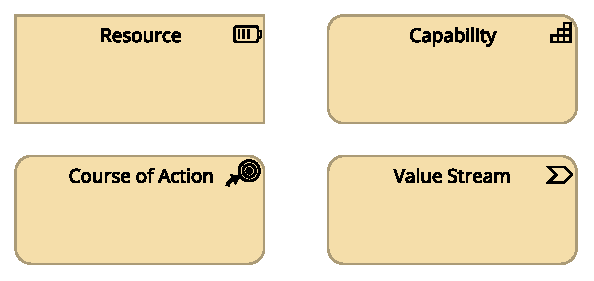
\includegraphics[width=\linewidth]{strategy-legend.pdf}
    \column{0.5\textwidth}
    \footnotesize
    \begin{itemize}\setlength{\itemsep}{4pt}
      \item \textbf{Resource} -- aset berwujud/tak berwujud yang dimiliki
            organisasi.
      \item \textbf{Capability} -- kemampuan tingkat tinggi yang dituju.
      \item \textbf{Course of Action} -- pendekatan/rencana yang dipilih.
      \item \textbf{Value Stream} -- rangkaian tahap penciptaan nilai.
    \end{itemize}
  \end{columns}
  \takeaway{Elemen strategi memakai persegi panjang membulat berwarna kuning
  keemasan; ikon pojok membedakan jenisnya.}
\end{frame}

\begin{frame}{Membedakan Elemen Strategi}
  \vspace{6pt}
  \begin{itemize}
    \item \textbf{Sumber daya (resource):} aset yang dimiliki/dikendalikan
          (koneksi BI-FAST, platform API, keahlian tim).
    \item \textbf{Kapabilitas (capability):} kemampuan kasar dan stabil
          (``perpindahan dana'', ``kepatuhan'').
    \item \textbf{Arah tindakan (course of action):} pilihan beserta urutan dan
          prioritas.
    \item \textbf{Value stream:} alur nilai tingkat tinggi yang didukung
          kapabilitas.
  \end{itemize}
  \takeaway{Beda dengan lapisan bisnis: kapabilitas strategis \emph{kasar};
  proses bisnis \emph{merincinya} menjadi langkah konkret.}
\end{frame}

% ============================================================
\section{Membaca Strategi: Model Bisnis \& Operating Model}
\sectionframe{Membaca Strategi:\\ Model Bisnis \& Operating Model}

\begin{frame}{Operating Model: Empat Pola}
  \vspace{4pt}
  \centering
  \scalebox{0.82}{
    \begin{tikzpicture}[
      font=\small,
      axis/.style={-Latex, thick},
      cell/.style={draw, rounded corners=1.5mm, align=center,
        minimum width=40mm, minimum height=18mm},
    ]
      \draw[axis] (0,0) -- (9,0) node[right] {\footnotesize\textbf{Integrasi data tinggi}};
      \draw[axis] (0,0) -- (0,5.2) node[above, align=center]
        {\footnotesize\textbf{Standardisasi}\\\footnotesize\textbf{proses tinggi}};
      \node[cell, fill=gray!12] (div) at (2.3,1.3) {\textbf{Diversification}};
      \node[cell, fill=blue!12] (coord) at (6.7,1.3) {\textbf{Coordination}};
      \node[cell, fill=orange!18] (rep) at (2.3,3.9) {\textbf{Replication}};
      \node[cell, fill=praditagreen!28, line width=0.5mm, draw=praditagreen]
        (uni) at (6.7,3.9) {\textbf{Unification}\\\footnotesize proses \& data seragam};
    \end{tikzpicture}
  }

  \takeaway{Rel transfer menuntut \textbf{Unification}: proses konsisten lintas
  kanal dan data nasabah terpadu agar limit \& AML
  (\emph{anti-money laundering}) otomatis.}
\end{frame}

\begin{frame}{Dari Model Bisnis ke Kapabilitas}
  \vspace{6pt}
  \begin{itemize}
    \item \textbf{Kanvas model bisnis} memetakan segmen pelanggan, proposisi
          nilai, aktivitas \& sumber daya kunci, dan mitra.
    \item Proposisi nilai ``perpindahan dana instan bagi UMKM'' $\rightarrow$
          kapabilitas \textbf{transfer} dan \textbf{kemitraan API} menjadi
          aktivitas serta sumber daya kunci.
    \item \emph{Operating model} menjelaskan tingkat standardisasi proses dan
          integrasi data yang dibutuhkan agar strategi dapat dijalankan.
  \end{itemize}
  \takeaway{Model bisnis dan operating model adalah \emph{alat baca} untuk
  membenarkan arah tindakan---bukan sekadar pelengkap.}
\end{frame}

% ============================================================
\section{TOGAF-lite dan Visi Arsitektur}
\sectionframe{TOGAF-lite dan Visi Arsitektur}

\begin{frame}{ADM-lite: Enam Pertanyaan}
  \vspace{6pt}
  \centering
  \scalebox{0.82}{
    \begin{tikzpicture}[
      box/.style={rectangle, rounded corners=1.5mm, draw=praditagreen,
        fill=praditagreen!10, thick, align=center, text width=26mm,
        minimum height=11mm, font=\footnotesize},
      flow/.style={-Latex, thick, draw=praditagreen},
      note/.style={rectangle, rounded corners=1.5mm, draw=gray!50,
        fill=gray!10, align=center, text width=28mm, minimum height=9mm,
        font=\footnotesize}
    ]
      \node[box] (problem) {Masalah \&\\pertanyaan riset};
      \node[box, right=6mm of problem] (vision) {Visi\\arsitektur};
      \node[box, right=6mm of vision] (baseline) {Kondisi\\saat ini};
      \node[box, below=20mm of baseline] (target) {Kondisi\\target};
      \node[box, left=6mm of target] (gap) {Analisis\\kesenjangan};
      \node[box, left=6mm of gap] (roadmap) {Rekomendasi\\\& roadmap};
      \draw[flow] (problem) -- (vision);
      \draw[flow] (vision) -- (baseline);
      \draw[flow] (baseline) -- (target);
      \draw[flow] (target) -- (gap);
      \draw[flow] (gap) -- (roadmap);
      \draw[flow] (roadmap.west) .. controls +(-8mm,5mm) and +(-8mm,-5mm) ..
        (problem.west);
      \node[note, below=5mm of vision] (evidence) {Tinjauan pustaka\\\& bukti};
      \draw[flow, dashed] (evidence) -- (vision);
      \draw[flow, dashed] (evidence) -- (gap);
    \end{tikzpicture}
  }
  
  \takeaway{TOGAF-lite = ambil \emph{pola berpikir} ADM, bukan seluruh
  dokumentasi. Pustaka memperkuat visi dan analisis kesenjangan.}
\end{frame}

\begin{frame}{Visi Arsitektur}
  \vspace{2pt}
  \footnotesize
  \begin{columns}[t]
    \column{0.5\textwidth}
    \textbf{Apa \& Mengapa}
    \begin{itemize}\setlength{\itemsep}{2.5pt}
      \item Pernyataan awal \emph{arah perubahan} yang ingin dicapai.
      \item Menjawab: masalah apa yang diubah, hasil apa yang diharapkan, batas
            mana yang tidak dibahas.
      \item Menyebut pemangku kepentingan utama dan arah tindakan strategis.
      \item Memberi arah yang cukup jelas untuk \emph{dianalisis}, bukan slogan.
    \end{itemize}
    \column{0.5\textwidth}
    \textbf{Bagaimana (Bank Wanua)}
    \begin{enumerate}\setlength{\itemsep}{2.5pt}
      \item \textbf{Masalah}: sasaran transfer real-time belum didukung rel yang
            terkelola \& patuh.
      \item \textbf{Arah tindakan}: bangun rel transfer (bungkus BI-FAST) lebih
            dahulu.
      \item \textbf{Hasil}: transfer 24/7 dengan penyaringan \& rekonsiliasi
            otomatis.
      \item \textbf{Batas}: bukan penggantian \emph{core banking}.
    \end{enumerate}
  \end{columns}
  \vspace{2pt}
  \takeaway{Visi membatasi lingkup makalah dan menjadi bahan langsung
  \textbf{Pendahuluan} dan \textbf{Metode}.}
\end{frame}

% ============================================================
\section{Studi Kasus: Strategi API Transfer Bank Wanua}
\sectionframe{Studi Kasus:\\ Strategi API Transfer Bank Wanua}

\begin{frame}{Peta Jalan Kapabilitas Digital UMKM}
  \vspace{2pt}
  \scriptsize
  \setlength{\extrarowheight}{2pt}
  \arrayrulecolor{black}\setlength{\arrayrulewidth}{0.5pt}
  \begin{tabularx}{\textwidth}{|p{0.12\textwidth}|p{0.34\textwidth}|X|}
    \hline
    \rowcolor{praditagreen!18}
    \textbf{Prioritas} & \textbf{Kapabilitas / API} & \textbf{Alasan Strategis} \\
    \hline
    P1 & Single-view nasabah UMKM & Fondasi data; menutup kesenjangan terbesar. \\
    \hline
    P1 & Onboarding digital \& e-KYC & Pintu masuk value stream; bergantung kepatuhan. \\
    \hline
    \rowcolor{orange!18}
    P1--P2 & \textbf{API Transfer Dana (rel)} & Rel primitif pembungkus BI-FAST; fondasi semua perpindahan dana. \\
    \hline
    P2 & API penerimaan (QRIS/VA) & Magnet UMKM, tetapi menumpuk pada rel transfer. \\
    \hline
    P3--P4 & Kredit, analitik, portal mitra & Bertumpu pada data \& transaksi inti. \\
    \hline
  \end{tabularx}
  \vspace{4pt}
  \takeaway{Arah tindakan: \textbf{rel transfer lebih dahulu}, baru layanan di
  atasnya---fondasi sebelum yang ``terlihat menarik''.}
\end{frame}

\begin{frame}{Visi Arsitektur Rel Transfer Bank Wanua}
  \vspace{6pt}
  \footnotesize
  \begin{quote}
  Bank Wanua membutuhkan rel perpindahan dana terkelola yang membungkus BI-FAST
  dan dibuka sebagai API yang patuh SNAP BI (Standar Nasional Open API
  Pembayaran), sehingga layanan transfer \emph{real-time} dapat diluncurkan
  bertahap ke kanal digital dan mitra UMKM tanpa mengabaikan keamanan,
  penyaringan kepatuhan, dan keberlanjutan sistem inti yang ada.
  \end{quote}
  \vspace{2pt}
  \begin{itemize}\setlength{\itemsep}{2pt}
    \item \textbf{Fokus}: membangun rel transfer \emph{di atas} core, bukan
          mengganti core.
    \item \textbf{Nilai}: percepatan dan keandalan perpindahan dana bagi UMKM.
    \item \textbf{Urutan}: transfer dahulu, pembayaran kemudian.
  \end{itemize}
  \takeaway{Visi memuat keputusan strategis yang dapat ditelusuri ke lapisan
  motivasi.}
\end{frame}

\begin{frame}{}
  \centering
  \vspace{1mm}
  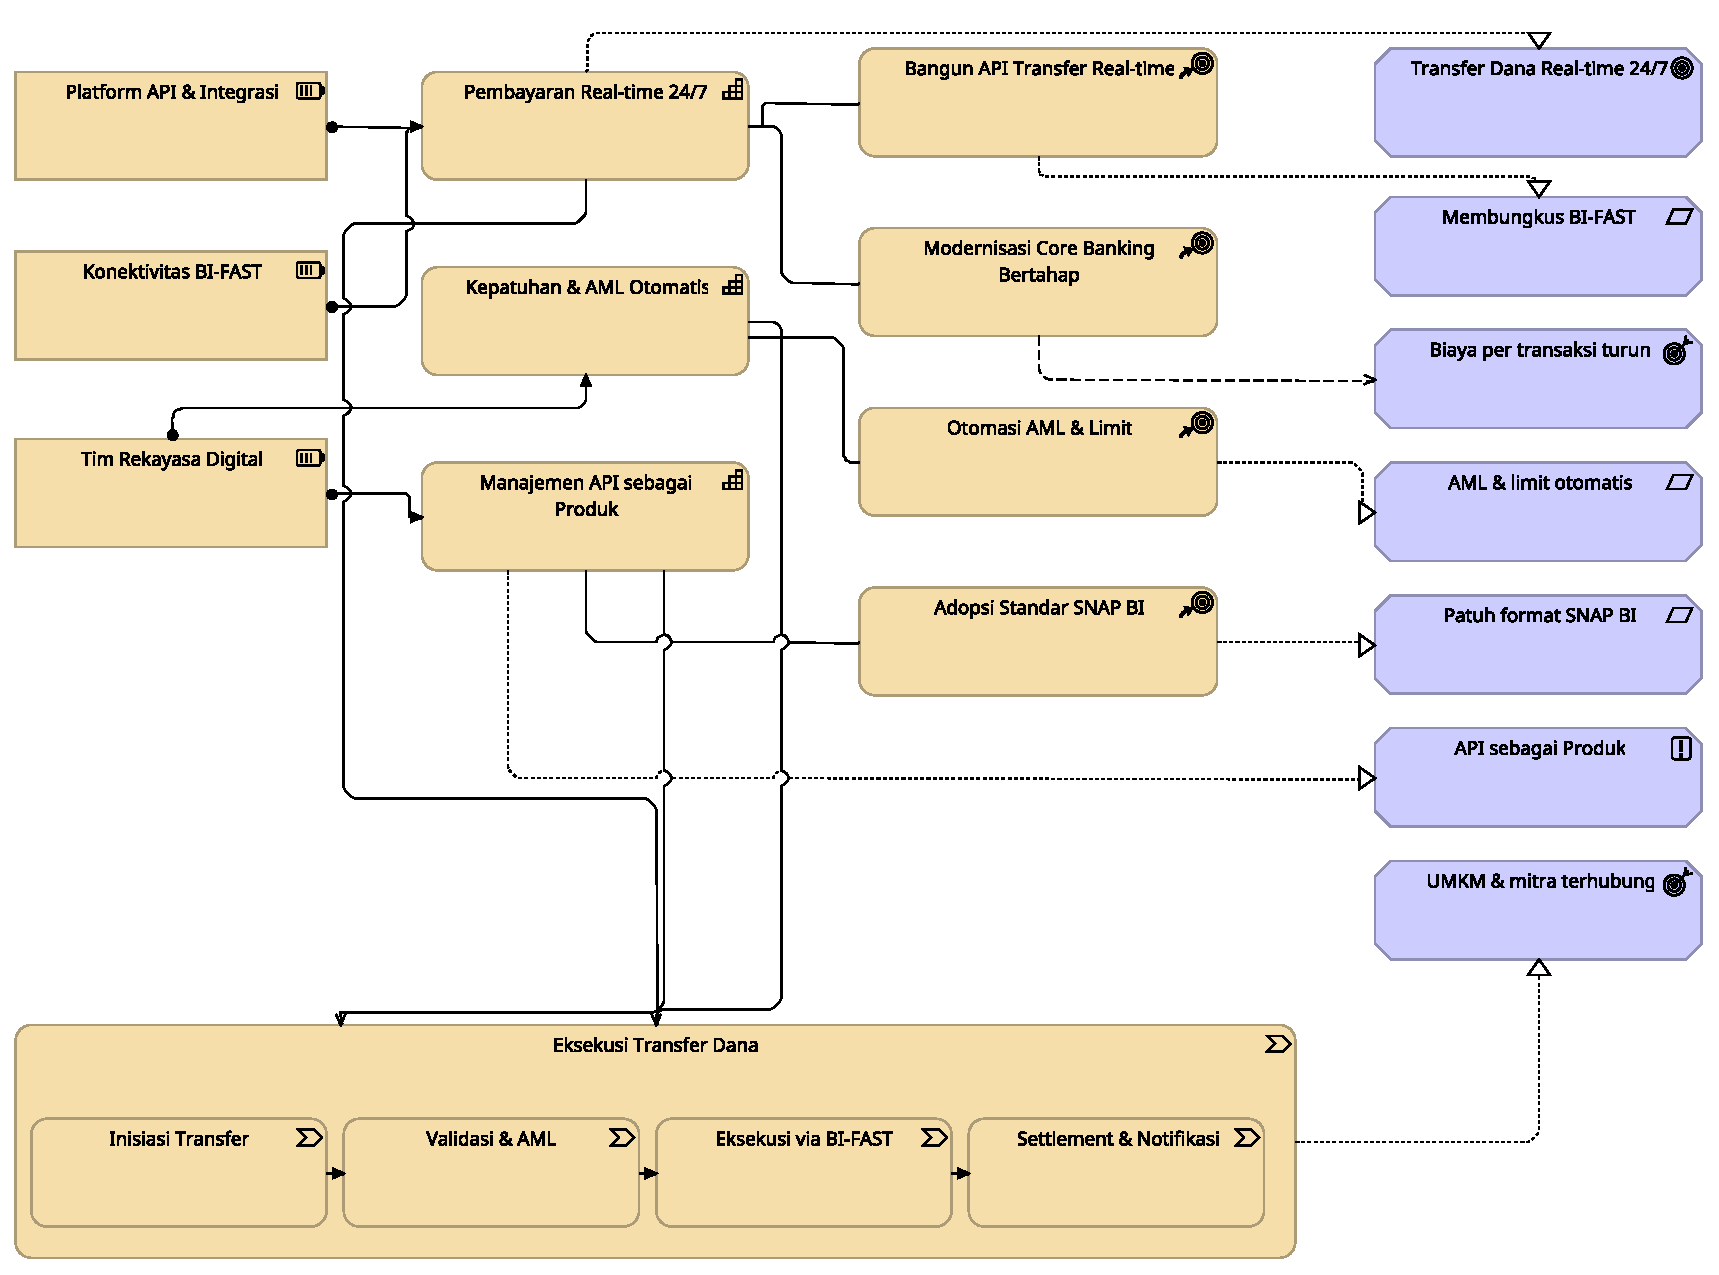
\includegraphics[height=.9\textheight]{strategy-transfer.pdf}\\
  {\scriptsize Model Strategi ArchiMate API Transfer Dana---diturunkan dari
  lapisan motivasi, dibangun dengan Archi.}
\end{frame}

\begin{frame}{Cara Membaca Diagram Strategi}
  \vspace{4pt}
  \footnotesize
  Dibaca kiri ke kanan: \textbf{sumber daya} $\rightarrow$ \textbf{kapabilitas}
  $\rightarrow$ \textbf{arah tindakan} $\rightarrow$ elemen \textbf{motivasi}.
  \begin{itemize}\setlength{\itemsep}{2.5pt}
    \item \textbf{Penugasan} (assignment): sumber daya (platform API, koneksi
          BI-FAST, tim) ditugaskan ke kapabilitas.
    \item \textbf{Asosiasi}: tiap arah tindakan menyatakan kapabilitas yang
          dibutuhkannya.
    \item \textbf{Realisasi}: arah tindakan merealisasikan \emph{kebutuhan}
          (bungkus BI-FAST, AML otomatis, patuh SNAP); kapabilitas
          merealisasikan \emph{sasaran} \& \emph{prinsip}.
    \item \textbf{Layanan \& pengaruh}: kapabilitas melayani value stream;
          modernisasi core memengaruhi \emph{biaya turun}.
  \end{itemize}
  \takeaway{Value stream \textbf{Eksekusi Transfer Dana} terinci menjadi empat
  tahap: Inisiasi $\rightarrow$ Validasi \& AML $\rightarrow$ Eksekusi via
  BI-FAST $\rightarrow$ Settlement \& Notifikasi.}
\end{frame}

% ============================================================
\section{Tinjauan Pustaka \& Bibliografi}
\sectionframe{Tinjauan Pustaka \& Bibliografi}

\begin{frame}{Strategi Pencarian Pustaka}
  \vspace{6pt}
  \begin{itemize}
    \item Mulai dari konsep utama pertanyaan riset; padankan istilah global
          dan Indonesia.
    \item Kata kunci: \emph{enterprise architecture}, \emph{API governance},
          \emph{payment/transfer API}, \emph{open banking},
          \emph{legacy modernization}, \emph{digital platform}.
    \item Padanan: ``arsitektur enterprise'', ``tata kelola API'', ``layanan
          transfer dana''.
    \item Bibliografi awal: minimal \textbf{sepuluh} rujukan bermakna, tiap
          sumber diberi alasan pemakaian.
  \end{itemize}
  \takeaway{Tinjauan pustaka = menunjukkan pemahaman atas percakapan ilmiah,
  bukan kumpulan ringkasan artikel.}
\end{frame}

\begin{frame}{Matriks Sintesis}
  \vspace{6pt}
  \begin{itemize}
    \item Membandingkan sumber, \emph{bukan} meringkas satu per satu.
    \item Kolom: definisi, peran ekosistem, mekanisme tata kelola, implikasi
          arsitektur, dan celah riset.
    \item Hubungan antar-konsep (platform, API, operating model, EA) menjadi
          \textbf{kerangka konseptual} makalah.
  \end{itemize}
  \takeaway{Dari pustaka ke kerangka konseptual: yang dinilai adalah
  \emph{hubungan} antar-sumber, bukan jumlahnya.}
\end{frame}

% ============================================================
\section{Latihan dan Jembatan}
\sectionframe{Latihan dan Jembatan}

\begin{frame}{Latihan Terapan Individual}
  \vspace{8pt}
  \begin{itemize}
    \item \textbf{Latihan 4.1} -- Arah tindakan dan peta jalan (min.\ tiga
          tingkat prioritas) untuk organisasi Anda.
    \item \textbf{Latihan 4.2} -- Visi arsitektur satu halaman.
    \item \textbf{Latihan 4.3} -- Strategi pencarian \& bibliografi awal (min.\
          sepuluh referensi).
    \item \textbf{Latihan 4.4} -- Matriks sintesis \& paragraf metode
          (TOGAF-lite operasional).
  \end{itemize}
  \takeaway{Semua latihan menjadi bahan langsung Tinjauan Pustaka, Kerangka
  Konseptual, dan Metode makalah.}
\end{frame}

\begin{frame}{Jembatan ke Bab Berikutnya}
  \vspace{8pt}
  \begin{itemize}
    \item Bab berikutnya turun ke \textbf{lapisan bisnis}: layanan, proses,
          peran, dan value stream bisnis yang mewujudkan rel transfer.
    \item Kapabilitas strategis ``perpindahan dana'' akan \emph{dirinci} menjadi
          proses dan layanan konkret.
    \item Visi arsitektur dan peta jalan memandu pemilihan proses yang dibedah.
  \end{itemize}
  \takeaway{Strategi yang jelas adalah kompas bagi rancangan bisnis, aplikasi,
  dan teknologi berikutnya.}
\end{frame}

\begin{frame}{\hfill}
  \centering
  \Huge{\textbf{Terima kasih}}\\[8pt]
  \normalsize Pertanyaan \& diskusi
\end{frame}

\end{document}
